% -*- latex -*-
%%%%%%%%%%%%%%%%%%%%%%%%%%%%%%%%%%%%%%%%%%%%%%%%%%%%%%%%%%%%%%%%
%%%%%%%%%%%%%%%%%%%%%%%%%%%%%%%%%%%%%%%%%%%%%%%%%%%%%%%%%%%%%%%%
%%%%
%%%% This text file is part of the source of 
%%%% `Parallel Computing'
%%%% by Victor Eijkhout, copyright 2012-5
%%%%
%%%% mpi.tex : leftover MPI topics
%%%%
%%%%%%%%%%%%%%%%%%%%%%%%%%%%%%%%%%%%%%%%%%%%%%%%%%%%%%%%%%%%%%%%
%%%%%%%%%%%%%%%%%%%%%%%%%%%%%%%%%%%%%%%%%%%%%%%%%%%%%%%%%%%%%%%%

\Level 0 {Synchronization}
\index{synchronization!in MPI|(}

MPI programs conform to the \ac{SPMD} model, and this means that events
in one process can be unrelated in time to events in another process.
Any \emph{synchronization} that happens is induced by communication 
and other MPI mechanisms. By synchronization here we mean any sort of
temporal ordering of events in different processes.

You have already seen some mechanisms.
\begin{enumerate}
\item In blocking communication, the receive call does not return until the send call has completed.
\item In non-blocking communication, the wait on a receive request will not return 
  until the send has been completed.
\item In one-sided communication, the fence mechanism impose a certain ordering on events.
\end{enumerate}

Another synchronization mechanism is induced by the \emph{barrier}\index{barrier!in MPI}
mechanism. However, while an \indexmpishow{MPI_Barrier} call guarantees that all processes have
reached a certain location in their source, this does not necessarily imply anything about 
message traffic. Consider this example
\begin{quotation}
  \begin{tabular}{|l|l|l|}
    \hline
    Proc 0 & Proc 1 & Proc 2\\
    \hline
    Isend to 1 & Irecv from any source & \\
    Barrier    & Barrier               & Barrier \\
    Wait for send request & wait for recv request & Isend to 1 \\
                          & (another wildcard recv) & wait for send request \\
    \hline
  \end{tabular}
\end{quotation}
The unexpected behaviour here is that the (first) receive on process~1
can be matched with the send on process~2: the barrier on process~1 only guarantees that the 
receive instruction was performed, not the actual transfer. For that you need the \n{MPI_Wait}
call, which is after the barrier.

\index{synchronization!in MPI|)}

\Level 0 {Hybrid programming: MPI and threads}\
\commandref{mpi-thread}

It is not automatic that a program or a library is
\indexterm{thread-safe}.  A user can request a certain level of
multi-threading with \indexmpishow{MPI_Init_thread}, and the system
will respond what the highest supported level is.

MPI can be thread-safe on the following levels:
\begin{itemize}
\item An MPI implementation can forbid any multi-threading;
\item it can allow one thread to make MPI calls;
\item it can allow one thread \emph{at a time} to make MPI calls;
\item it can allow arbitrary multi-threaded behaviour in MPI calls.
\end{itemize}

Some points.
\begin{itemize}
\item MPI can not distinguish between threads: the communicator rank
  identifies a process, and is therefore identical for all threads.
\item A message sent to a process can be received by any thread that
  has issued a receive call with the right source/tag specification.
\item Multi-threaded calls to an MPI routine have the semantics of an
  unspecified sequence of calls.
\item A blocking MPI call only blocks the thread that makes it.
\end{itemize}

\Level 0 {Leftover topics}

\Level 1 {Getting message information}

In some circumstances the recipient may not know all details of a message.
\begin{itemize}
\item If you are expecting multiple incoming messages, it may be most
  efficient to deal with them in the order in which they arrive. For
  that, you have to be able to ask `who did this message come from,
  and what is in it'.
\item Maybe you know the sender of a message, but the amount of data
  is unknown. In that case you can overallocate your receive buffer,
  and after the message is received ask how big it was, or you can
  `probe' an incoming message and allocate enough data when you find
  out how much data is being sent.
\end{itemize}

\Level 2 {Status object}

The receive calls you saw above has a status argument. If you 
precisely know what is going to be sent, this argument tells you 
nothing new. Therefore, there is a special value \indexmpishow{MPI_STATUS_IGNORE}
that you can supply instead of a status object, which tells MPI that the 
status does not have to be reported. For routines such as \indexmpishow{MPI_Waitany}
where an array of statuses is needed, you can supply \indexmpishow{MPI_STATUSES_IGNORE}.

However, if you expect data from multiple senders,
or the amount of data is indeterminate, the status will give
you that information.

The \indexmpishow{MPI_Status} object is a structure with the following 
freely accessible members:
\n{MPI_SOURCE}, \n{MPI_TAG}, and \n{MPI_ERROR}. There is also opaque 
information: the amount of data received can be retrieved by 
a function call to \indexmpishow{MPI_Get_count}.
\begin{verbatim}
int MPI_Get_count(
  MPI_Status *status,
  MPI_Datatype datatype,
  int *count
);
\end{verbatim}
This may be necessary since the \n{count} argument to \n{MPI_Recv} is 
the buffer size, not an indication of the actually expected number of
data items.

\Level 1 {Error handling}
\commandref{mpi:error}

Errors in normal programs can be tricky to deal with; errors in
parallel programs can be even harder. This is because in addition to
everything that can go wrong with a single executable (floating point
errors, memory violation) you now get errors that come from faulty
interaction between multiple executables.

A few examples of what can go wrong:
\begin{itemize}
\item MPI errors: an MPI routine can abort for various reasons, such
  as receiving much more data than its buffer can accomodate. Such
  errors, as well as the more common type mentioned above, typically
  cause your whole execution to abort. That is, if one incarnation of
  your executable aborts, the MPI runtime will kill all others.
\item Deadlocks and other hanging executions: there are various
  scenarios where your processes individually do not abort, but are all
  waiting for each other. This can happen if two processes are both
  waiting for a message from each other, and this can be helped by
  using non-blocking calls. In another scenario, through an error in
  program logic, one process will be waiting for more messages
  (including non-blocking ones) than are sent to it.
\end{itemize}

The MPI library has a general mechanism for dealing with errors that
it detects. The default behaviour, where the full run is aborted, is
equivalent to your code having the following
call\indexmpi{MPI_Comm_set_errhandler}\footnote{The routine
  \n{MPI\_Errhandler\_set} is deprecated.}:
\indexmpi{MPI_ERRORS_ARE_FATAL}\indexmpi{MPI_ERRORS_RETURN}
\begin{verbatim}
MPI_Comm_set_errhandler(MPI_COMM_WORLD,MPI_ERRORS_ARE_FATAL);
\end{verbatim}
Another simple possibility is to specify
\begin{verbatim}
MPI_Comm_set_errhandler(MPI_COMM_WORLD,MPI_ERRORS_RETURN);
\end{verbatim}
which gives you the opportunity to write code that handles the error
return value.

In most cases where an MPI error occurs a complete abort is the
sensible thing, since there are few ways to recover. The second
possibility can for instance be used to print out debugging
information:
\begin{verbatim}
ierr = MPI_Something();
if (ierr!=0) {
    // print out information about what your programming is doing
    MPI_Abort();
}
\end{verbatim}
For instance,
\begin{verbatim}
Fatal error in MPI_Waitall: 
See the MPI_ERROR field in MPI_Status for the error code
\end{verbatim}
You could code this as\indexmpi{MPI_Error_string}\indexmpi{MPI_ERROR}
\begin{verbatim}
MPI_Comm_set_errhandler(MPI_COMM_WORLD,MPI_ERRORS_RETURN);
ierr = MPI_Waitall(2*ntids-2,requests,status);
if (ierr!=0) {
   char errtxt[200];
   for (int i=0; i<2*ntids-2; i++) {
       int err = status[i].MPI_ERROR; int len=200;
       MPI_Error_string(err,errtxt,&len);
       printf("Waitall error: %d %s\n",err,errtxt);
   }
   MPI_Abort(MPI_COMM_WORLD,0);
}
\end{verbatim}
One cases where errors can be handled is that of \emph{MPI file
  I/O}\indexterm{MPI!I/O}: if an output file has the wrong
permissions, code can possibly progress without writing data, or
writing to a temporary file.

\Level 1 {Fortran issues}
\commandref{mpi-fortran}
\index{MPI!Fortran issues|(}

MPI is typically written in C, what if you program \emph{Fortran}?

Assumed shape arrays can be a problem: they need to be copied. 
That's a problem with Isend.

\begin{itemize}
\item Fortran routines have the same prototype as C~routines except for the addition
  of an integer error parameter.
\item The call for \indexmpishowsub{MPI_Init}{in Fortran} does not have the commandline arguments;
  they need to be handled separately.
\item The routine \indexmpishow{MPI_Sizeof} is only available in Fortran, it provides the 
  functionality of the C/C++ operator \indextermtt{sizeof}.
\end{itemize}

\index{MPI!Fortran issues|)}

\Level 1 {Fault tolerance}
\label{mpi:tolerant}

Processors are not completely reliable, so it may happen that one
`breaks': for software or hardware reasons it becomes
unresponsive. For an MPI program this means that it becomes impossible
to send data to it, and any collective operation involving it will
hang. Can we deal with this case? Yes, but it involves some
programming.

First of all, one of the possible MPI error return codes
(section~\ref{mpi:error}) is \n{MPI_ERR_COMM}, which can be returned
if a processor in the communicator is unavailable. You may want to
catch this error, and add a `replacement processor' to the
program. For this, the \n{MPI_Comm_spawn} can be used:
\begin{verbatim}
int MPI_Comm_spawn(char *command, char *argv[], int maxprocs, MPI_Info info, 
                  int root, MPI_Comm comm, MPI_Comm *intercomm,
                  int array_of_errcodes[])
\end{verbatim}
But this requires a change of program design: the communicator
containing the new process(es) is not part of the
old \n{MPI_COMM_WORLD}, so it is better to set up your code as a
collection of inter-communicators to begin with.

\Level 1 {Context information}
\commandref{context}

The \indextermbus{MPI}{version} is available through two parameters
\indexmpishow{MPI_VERSION} and \indexmpishow{MPI_SUBVERSION}
or the function \indexmpishow{MPI_Get_version}.

\Level 1 {Timing}
\commandref{mpi-timing}
\index{timing!MPI|(}

Timing of parallel programs is tricky. On each node you can use a timer,
typically based on some \ac{OS} call. MPI supplies its own routine
\indexmpishow{MPI_Wtime} which gives \indexterm{wall clock time}.
Normally you don't worry about the starting point for this timer: 
you call it before and after an event and subtract the values.
\begin{verbatim}
t = MPI_Wtime();
// something happens here
t = MPI_Wtime()-t;
\end{verbatim}
If you execute this on a single processor you get fairly reliable
timings, except that you would need to subtract the overhead for the
timer. This is the usual way to measure timer overhead:
\begin{verbatim}
t = MPI_Wtime();
// absolutely nothing here
t = MPI_Wtime()-t;
\end{verbatim}

\Level 2 {Global timing}

However, if you try to time a parallel application you will most likely
get different times for each process, so you would have to take the
average or maximum.  Another solution is to synchronize the processors
by using a \indexterm{barrier}\indexmpi{MPI_Barrier}:
\begin{verbatim}
MPI_Barrier(comm)
t = MPI_Wtime();
// something happens here
MPI_Barrier(comm)
t = MPI_Wtime()-t;
\end{verbatim}

\begin{exercise}
  This scheme also has some overhead associated with it. How would you measure that?
\end{exercise}

\Level 2 {Local timing}
\label{sec:ping-time}

Now suppose you want to measure the time for a single send. It is not possible
to start a clock on the sender and do the second measurement on the receiver,
because the two clocks need not be synchronized. Usually a \indexterm{ping-pong} is 
done: 
\begin{verbatim}
if ( proc_source ) {
  MPI_Send( /* to target */ );
  MPI_Recv( /* from target */ );
else if ( proc_target ) {
  MPI_Recv( /* from source */ );
  MPI_Send( /* to source */ );
}
\end{verbatim}

\begin{exercise}
  Why is it generally not a good idea to use processes 0 and~1 for the
  source and target processor?  Can you come up with a better guess?
\end{exercise}

No matter what sort of timing you are doing, it is good to know the accuracy of your timer.
The routine \indexmpishow{MPI_Wtick} gives the smallest possible timer increment.
If you find that your timing result is too close to this `tick', you need to find a better timer
(for CPU measurements there are cycle-accurate timers), or you need to increase
your running time, for instance by increasing the amount of data.

\index{timing!MPI|)}

\Level 1 {Profiling}
\commandref{profile}

MPI allows you to write your own profiling interface. To make this possible,
every routine \n{MPI_Something} calls a routine \n{PMPI_Something} that 
does the actual work. You can now write your \n{MPI_...} routine
which calls \indexmpishow{PMPI_...}, and inserting your own profiling calls.
\begin{figure}
  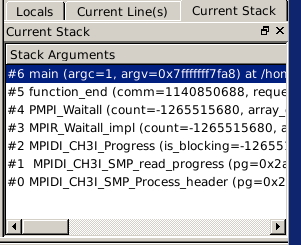
\includegraphics[scale=.7]{graphics/pmpi}
  \caption{A stack trace, showing the \texttt{PMPI} calls.}
  \label{fig:pmpi}
\end{figure}
As you can see in figure~\ref{fig:pmpi}, normally only the \n{PMPI} routines
show up in the stack trace.

Does the standard mandate this?

\Level 1 {Debugging}
\label{sec:debug}

There are various ways of debugging an MPI program. Typically there
are two cases. In the simple case your program can have a serious
error in logic which shows up even with small problems and a small
number of processors. In the more difficult case your program can only
be run on large scale, or the problem only shows up when you run at
large scale. For the second case you, unfortunately, need a dedicated
debugging tool, and of course the good ones are expensive. In the
first case there are some simpler solutions.

\Level 2 {Small scale debugging}

If your program hangs or crashes even with small numbers of
processors, you can try debugging on your local desktop or laptop
computer:
\begin{verbatim}
mpirun -np <n> xterm -e gdb yourprogram
\end{verbatim}
This starts up a number of X~terminals, each of which runs your
program. The magic of \n{mpirun} makes sure that they all collaborate
on a parallel execution of that program. If your program needs
commandline arguments, you have to type those in every xterm:
\begin{verbatim}
run <argument list>
\end{verbatim}
See appendix~\ref{tut:debug} for more about debugging with~\n{gdb}.

This approach is not guaranteed to work, since it depends on
your \n{ssh} setup; see the discussion
in \url{http://www.open-mpi.org/faq/?category=debugging#serial-debuggers}.

\Level 2 {Large scale debugging}

Check out \indexterm{ddt} or \indexterm{TotalView}.

\Level 2 {Memory debugging of MPI programs}

The commercial parallel debugging tools typically have a memory
debugger. For an open source solution you can
use \indexterm{valgrind}, but that requires some setup during
installation. See \url{http://valgrind.org/docs/manual/mc-manual.html#mc-manual.mpiwrap}
for details.

\Level 1 {Determinism}
\label{sec:mpi-semantics}
\index{MPI!semantics|(}

MPI processes are only synchronized to a certain extent, so you may
wonder what guarantees there are that running a code twice will give
the same result.  You need to consider two cases: first of all, if the
two runs are on different numbers of processors there are already
numerical problems; see~\HPSCref{sec:roundoff-parallel}.

Let us then limit ourselves to two runs on the same set of processors. 
In that case, MPI is deterministic as long as you do not use 
wildcards such as \indexmpishow{MPI_ANY_SOURCE}. Formally, 
MPI messages are `non-overtaking': two messages between the same
sender-receiver pair will arrive in sequence.
Actually, they may not arrive in sequence: they are \emph{matched}\index{matching}
in sequence in the user program. If the second message is much smaller than the first,
it may actually arrive earlier in the lower transport layer.

\index{MPI!semantics|)}

\Level 1 {Progress}
\index{progress|(}

Non-blocking communication implies that messages make \emph{progress}
while computation is going on. However, communication of this sort can 
typically not be off-loaded to the network card, so it has to be done by 
a process. This requires a separate thread of execution, with
obvious performance problems. Therefore, in practice overlap may
not actually happen, and for the message to make progress
it is necessary for the MPI library to become active occasionally.
For instance, people have inserted dummy \n{MPI_Probe} calls.

A similar problem arises with passive target synchronization:
it is possible that the origin process may hang until 
the target process makes an MPI call.

\index{progress|)}

\Level 0 {Literature}

Online resources:
\begin{itemize}
\item MPI 1 Complete reference:\\ \url{http://www.netlib.org/utk/papers/mpi-book/mpi-book.html}
\item Official MPI documents:\\ \url{http://www.mpi-forum.org/docs/}
\item List of all MPI routines:\\ \url{http://www.mcs.anl.gov/research/projects/mpi/www/www3/}
\end{itemize}

Tutorial books on MPI:
\begin{itemize}
\item Using MPI~\cite{Gropp:UsingMPI1} by some of the original authors.
\end{itemize}

\endinput

Examples: 
compute pi
mandelbrot set
